\documentclass{article}

\usepackage{makecell}

% Document extensibility %
%
% Disables native paragraph indentation
\usepackage{parskip} 
%
% Provides further bullet options for lists
\usepackage{enumitem}

% Mathematical symbol and statement packages %
%
% Necessary
\usepackage{amsmath}
\usepackage{amssymb}
%
% Extensive fraction notation
\usepackage{xfrac}
%
% Generic mathematical commands
% Notable: \degree, \celcius
\usepackage{gensymb}
%
% Variable vector notation (arrow above variable)
\usepackage{esvect}
%
% Multiline boxed equations
\usepackage{empheq}
%
% SI Unit
\usepackage{siunitx}

% Graphic packages %
%
% Diagrams and illustrations
\usepackage{tikz}
%
% Image insertion
\usepackage{graphicx}
\graphicspath{ {./} }

% Document content %
%
% Change title of table of contents
% \renewcommand{\contentsname}{Title}

\begin{document}

% Command `\hr` to insert horizontal rules
\newcommand{\hr}{\par\noindent\rule{\textwidth}{0.4pt}}

% Command to box and center math equations
\newcommand{\bc}[1]{
	\begin{equation*}
		\begin{boxed}
			{#1}
		\end{boxed}
	\end{equation*}
}

\section{Cell Function: Diffusion and Osmosis}

\subsection{Procedure 1: Diffusion}
\textbf{DIFFUSION THROUGH A LIQUID}
\begin{enumerate}[label=\textbf{\arabic*.}]
	\item
	\item
		\SI{2.5}{\centi \meter}
	\item
		\SI{15}{\centi \meter \per \hour} \\
		\begin{tabular}{ c | c | c }
			Diffusion & Distance in \SI{10}{\minute} & Distance in \SI{1}{\hour} \\
			\hline
			Semi-solid & \SI{0.5}{\centi \meter} & \SI{3}{\centi \meter} \\
			Liquid & \SI{2.5}{\centi \meter} & \SI{15}{\centi \meter}
		\end{tabular}
	\item
		Liquid
	\item
		As gasses tend to be less dense than its counterparts, the movement and flow of solutes should be quicker resulting in a quicker rate of diffusion.
\end{enumerate}


\subsection{Procedure 2: Effect of Cell Size on Speed of Diffusion}
\begin{tabular}{ c | c | c | c | c | c }
	Cell & Dimensions & SA & Volume & SA : Volume & Total time \\
	\hline
	A & $ 1 \times 1 \times 1 $ & \SI{6}{\cm \squared} & \SI{1}{\cm \cubed} & $ 6 : 1 $ & \SI{10}{\minute} \\
	B & $ 2 \times 2 \times 2 $ & \SI{24}{\cm \squared} & \SI{8}{\cm \cubed} & 3 : 1 & \SI{1}{\hour} \SI{23}{\minute} \\
	C & $ 3 \times 3 \times 3 $ & \SI{54}{\cm \squared} & \SI{27}{\cm \cubed} & 2 : 1 & \SI{2}{\hour}
\end{tabular}

\begin{enumerate}[label=\textbf{\arabic*.}]
	\item
		Different sized cells
	\item
		The vinegar represents a solute that gradually diffuses its ``cell."
	\item
		So we can observe the diffusion taking place, and accurately record the time it takes.
	\item
		The change in color of the agar cube demonstrates that diffusion is occurring.
	\item
		The ratio of the surface area decreases in respect to the volume of the cell.
	\item
		The total time of diffusion gets longer.
\end{enumerate}

\subsection{Produce 3: Diffusion Across a Plasma Membrane}

\textbf{PREDICTION}

I believe that glucose, starch, and water will be able to pass across the cell membrane. This is due to their chemical density being similar and significantly less than iodine, which I believe will not pass across the cell membrane.

\begin{enumerate}[label=\textbf{\arabic*.}]
	\item
		Iodine is the indicator reagent for starch.
	\item
		By heating Benedict's solution, we can indicate the location of sugar.
	\item
		Iodine can be located by its amber color.
	\item
		Iodine and starch when combined turn to a darker color, and with the water being tainted with iodine, observing where there the darker color is present can help determine where the water moves.
	\item
	\item
		\begin{tabular}{ c | c | c }
			& Results/observations & Conclusions \\
			\hline
			Iodine & \makecell{Black particles \\ due to iodine} & \makecell{Iodine diffuses \\ across membrane \\ because of its small size} \\
			\hline
			Starch & \makecell{Starch and iodine \\ reaction inside of cell \\ membrane} & \makecell{The large density and size \\ of starch makes it unable \\ to difuse} \\
			\hline
			Glucose & Water turned orange & \makecell{The orange color in the \\ water signifies \\ glucose exiting the cell} \\
			\hline
			Water & \makecell{Weight decreased from \SI{28.95}{\gram} \\ to \SI{27.64}{\gram} $ \therefore $ water \\ left the cell membrane} & \makecell{Water exited \\ the cell membrane}
		\end{tabular}
\end{enumerate}

\subsection{Procedure 4: Osmosis}
\textbf{OSMOSIS IN POTATO CELLS}
\begin{enumerate}[label=\textbf{\arabic*.}]
	\item
	\item
		\begin{itemize}
			\item Initial Mass w/ 10\% Salt - \SI{0.05}{\gram}
			\item Initial Mass w/ Tap Water - \SI{0.06}{\gram}
		\end{itemize}
	\item
	\item
	\item
	\item
		\begin{tabular}{ c | c | c | c }
			Potato Tissue & Final Mass & Initial Mass & Net $ \pm $ of mass \\
			\hline
			Tap Water & \SI{7.27}{\gram} & \SI{0.05}{\gram} & \SI{7.22}{\gram} \\
			10\% Salt Water & \SI{6.93}{\gram} & \SI{0.06}{\gram} & \SI{6.87}{\gram}
		\end{tabular}
	\item
		Tap Water - Dense \& Firm \\
		10\% Salt Water - Soggy \& Flexible
\end{enumerate}

\textbf{QUESTIONS}
\begin{enumerate}[label=\textbf{\arabic*.}]
	\item
		Osmosis
	\item
		10\% Salt Water
	\item
		Tap Water
\end{enumerate}

\subsection{Procedure 5: Plasmolysis in Red Onion Skin Cells}
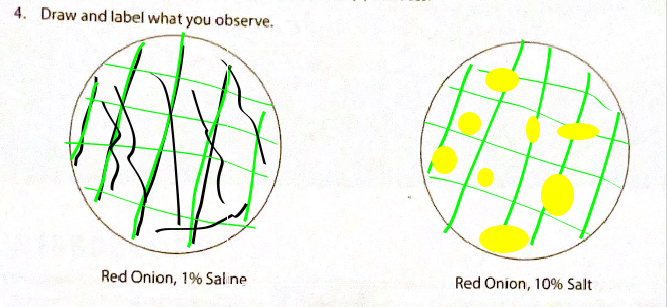
\includegraphics[width=\textwidth]{lab_four_image.png}
\textbf{QUESTIONS}
\begin{enumerate}[label=\textbf{\arabic*.}]
	\item
		After putting the salt water, I observed water exiting the onion skin and generally towards the outside demonstrating osmosis.
	\item
		10\% Salt
	\item
		1\% Saline
	\item
		Plant cells have cell walls which assist against diffusion in contrast to animal cells.
\end{enumerate}

\end{document}
